\section{Búsqueda de parámetros óptimos}

En esta sección diseñamos experimentos para encontrar parámetros óptimos de kNN y PCA de la herramienta de OCR implementado. Para poder hacer esto utilizamos el método de K-fold cross validation.

Las métricas utilizadas para analizar la calidad de los resultados del programa fueron: accuracy, precision, recall y F1 score.


\subsection{Hipótesis}
Para el algoritmo de KNN, nuestra hipótesis es que para los valores más bajos de $k$ la cantidad de aciertos será menor porque para caracteres similares una imagen puede tener algunos vecinos cercanos de otra clase. Luego, al tomar una poca cantidad de vecinos, se tomará a los que pertenecen a esta otra clase.

Para valores muy grandes de $k$, en cambio, se consideran demasiados vecinos haciendoq ue tome más importancia la cantidad de apariciones de un caracter que la cercanía de los miembros de su clase a la imagen a reconocer. Un ejemplo extremo que muestra claramente este comportamiento es cuando $k$ toma su valor máximo ---la cantidad total de datos de entrenamiento: la repuesta será siempre la clase que tenga más elementos en la base de entrenamiento.

Para el método de PCA, nuestra hipótesis es que la calidad de los resultados crecerá junto con el valor del parámetro $\alpha$ ---la cantidad de componentes principales a analizar. Sin embargo, creemos que existe un punto a partir del cual los resultados no van tener mejoras significativas debido a que la información adicional que aportan estas componentes será muy poca.

\subsection{Exploración manual de parámetros}

Como el tiempo de cómputo de los algoritmos son altos, primero se realizó una exploración manual con algunos parámetros dispersos con el fin de acotar el espacio de búsqueda.

En esta exploración se pudo notar que para valores de $\alpha$ mayores a $100$ la calidad de los resultados presentabas pocas diferencias. Por esto se decidió realizar una primera búsqueda con $\alpha \in \{1,5,10,20,30,50,100\}$ para $k \in \{1,5,10,20,30,50,100\}$.

Se pudo observar también en la exploración manual que la cantidad de folds utilizada en la validación cruzada no afectaba considerablemente los resultados obtenidos. Luego se limitó la validación al uso de 2, 5 y 10 folds.

\subsection{Primera búsqueda}

\subsubsection{Influencia de la cantidad de folds}

En primer lugar se puede observar que los resultados obtenidos o ---lo que es más importante--- la relación entre los mismos no es afectada significativamente por la cantidad de folds utilizados para la validación cruzada (figuras \ref{fig:cv_cmp_folds_accuracy}, \ref{fig:cv_cmp_folds_precision}, \ref{fig:cv_cmp_folds_recall}).

Por esto, entonces, se limitará el análisis a los resultados obtenidos en la validación con 5 folds.

\begin{figure}[h]
    \centering
    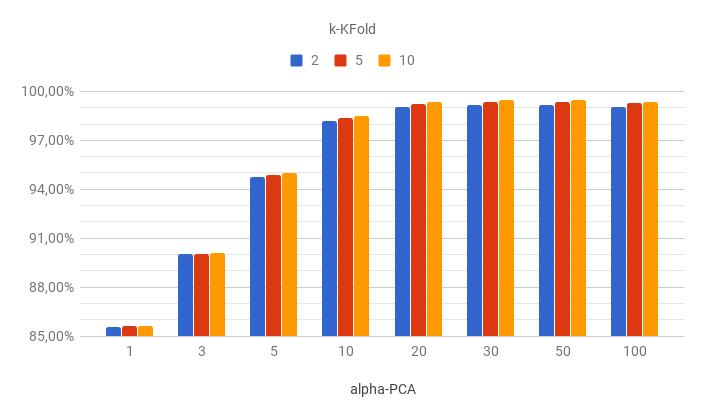
\includegraphics[width=\textwidth]{graficos/cv_cmp_folds_accuracy.png}
    \caption{Promedio de accuracy en función de alpha-PCA agrupado por k-KFold}
    \label{fig:cv_cmp_folds_accuracy}
\end{figure}

\begin{figure}[h]
    \centering
    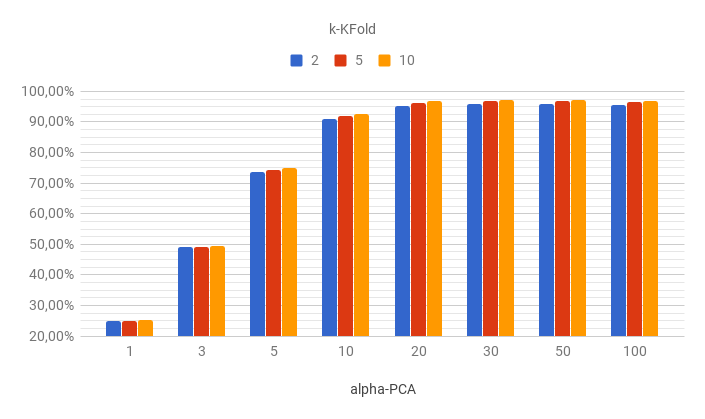
\includegraphics[width=\textwidth]{graficos/cv_cmp_folds_precision.png}
    \caption{Promedio de precision en función de alpha-PCA agrupado por k-KFold}
    \label{fig:cv_cmp_folds_precision}
\end{figure}

\begin{figure}[H]
    \centering
    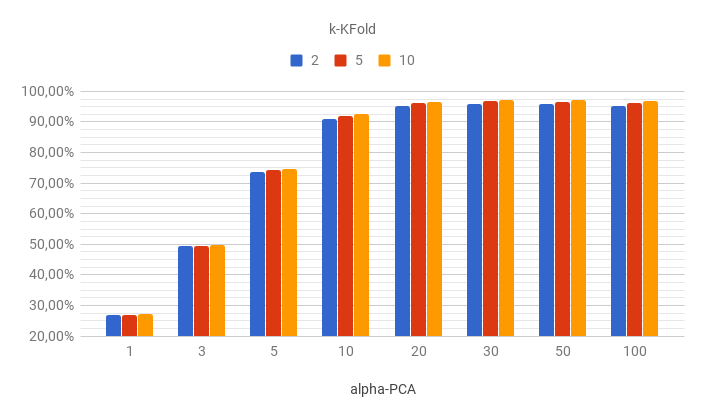
\includegraphics[width=\textwidth]{graficos/cv_cmp_folds_recall.png}
    \caption{Promedio de recall en función de alpha-PCA agrupado por k-KFold}
    \label{fig:cv_cmp_folds_recall}
\end{figure}

\subsubsection{Comparación de parámetros}

En cuanto al parámetro $\alpha$ se puede notar a primera vista en las figuras \ref{fig:cv1_accuracy}, \ref{fig:cv1_precision} y \ref{fig:cv1_recall} que, como se había planteado en la hipótesis, la calidad de los resultados crece junto con $\alpha$, pero existe un punto a partir del cual se estanca este crecimiento debido a que la información que aportan las componentes que se van agregando es muy poca. En este caso, dicho punto parece encontrarse alrededor de $\alpha = 20$. Se observa también que mejores resultados aparecen a partir de $\alpha = 10$.

\begin{figure}[h]
    \centering
    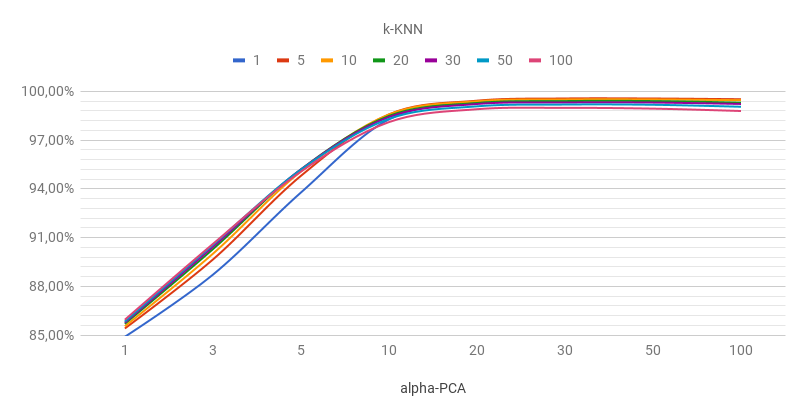
\includegraphics[width=\textwidth]{graficos/cv1_accuracy.png}
    \caption{Accuracy en función de alpha-PCA para cada k-KNN}
    \label{fig:cv1_accuracy}
\end{figure}

\begin{figure}[h]
    \centering
    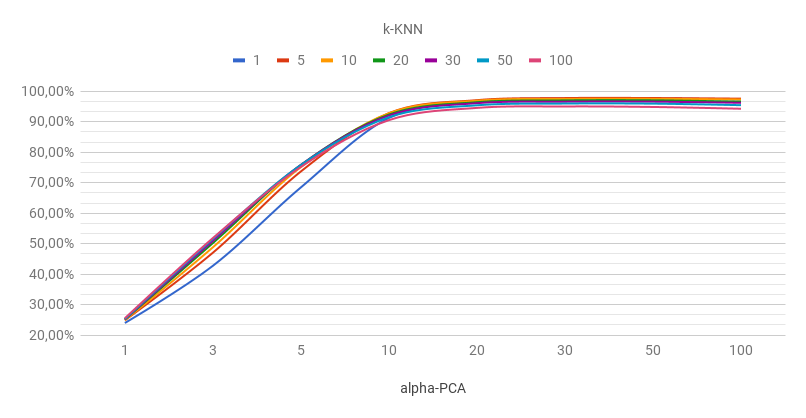
\includegraphics[width=\textwidth]{graficos/cv1_precision.png}
    \caption{Precision en función de alpha-PCA para cada k-KNN}
    \label{fig:cv1_precision}
\end{figure}

\begin{figure}[h]
    \centering
    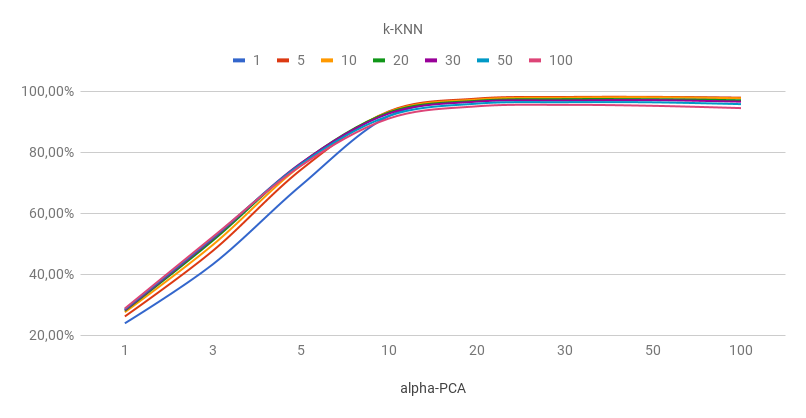
\includegraphics[width=\textwidth]{graficos/cv1_recall.png}
    \caption{Recall en función de alpha-PCA para cada k-KNN}
    \label{fig:cv1_recall}
\end{figure}

Mirando los gráficos más de cerca (figuras \ref{fig:cv1_accuracy_zoom}, \ref{fig:cv1_precision_zoom}, \ref{fig:cv1_recall_zoom}) se puede ver que los valores 1, 5 y 10 de k-KNN son los que tienen resultados superiores. Sorprendentemente, $k = 1$ es incluso mejor que $k = 10$. En la hipótesis se había mencionado que una imagen de una clase podía tener vecinos más cercanos de otra clase con similar escritura, por lo que valores muy pequeños de $k$ podrían seleccionar erróneamente a esta otra clase. Sin embargo, estos resultados sugieren que, para la base de entrenamiento usada, esta situación no se presenta muy frecuentemente.

Por otra parte, se ve claramente que luego de pasar el valor óptimo de $k$ la calidad de los resultados decrece a medida que aumenta la cantidad de vecinos considerados, como se esperaba.

Con respecto a $\alpha$ se observa que para los últimos valores medidos la calidad de los resultados empieza a decrecer, a diferencia de lo que se había dicho en la hipótesis. Una posible explicación que se pudo encontrar para este comportamiento considera el error inherente de la aritmética de números reales en una computadora:

El algoritmo de PCA obtiene de la matriz de covarianza los autovectores necesarios para determinar el cambio de base necesario. Para esto utiliza el método de la potencia, el cual realiza una serie de operaciones aritméticas de matrices por una cantidad determinada de iteraciones, introduciendo en cada iteración un error que se arrastra a las iteraciones siguientes. Luego de obtener cada autovector es necesario aplicar deflación para poder hallar el siguiente. En este procedimiento se utilizan este autovalor y autovector hallados. Esto implica que el cómputo de cada autovector arrastra los errores del cómputo de todos los autovectores anteriores. Luego, a medida que crece el valor de $\alpha$ este error se hace cada vez mayor, distorsionando cada vez más la información de las imágenes, lo que resulta en un decrecimiento de la calidad de los resultados.

\begin{figure}[h]
    \centering
    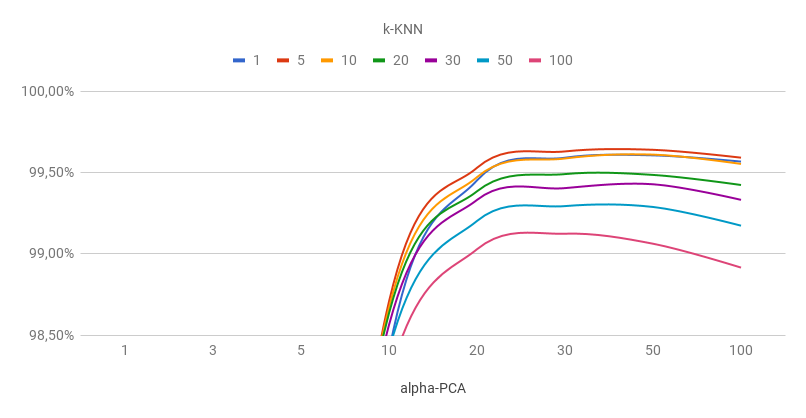
\includegraphics[width=\textwidth]{graficos/cv1_accuracy_zoom.png}
    \caption{Accuracy en función de alpha-PCA para cada k-KNN}
    \label{fig:cv1_accuracy_zoom}
\end{figure}

\begin{figure}[H]
    \centering
    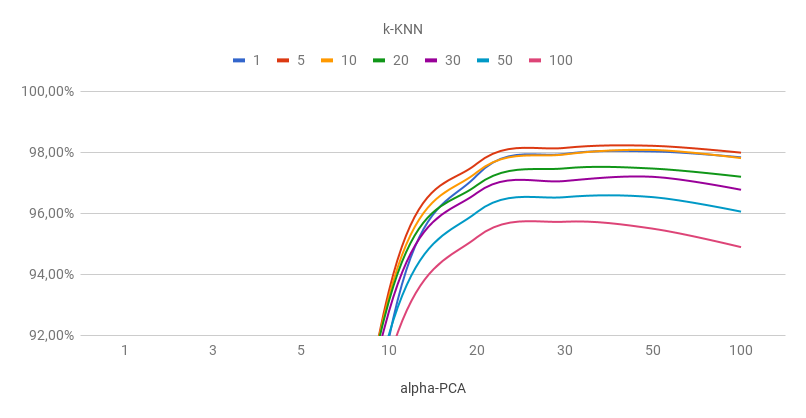
\includegraphics[width=\textwidth]{graficos/cv1_precision_zoom.png}
    \caption{Precision en función de alpha-PCA para cada k-KNN}
    \label{fig:cv1_precision_zoom}
\end{figure}

\begin{figure}[H]
    \centering
    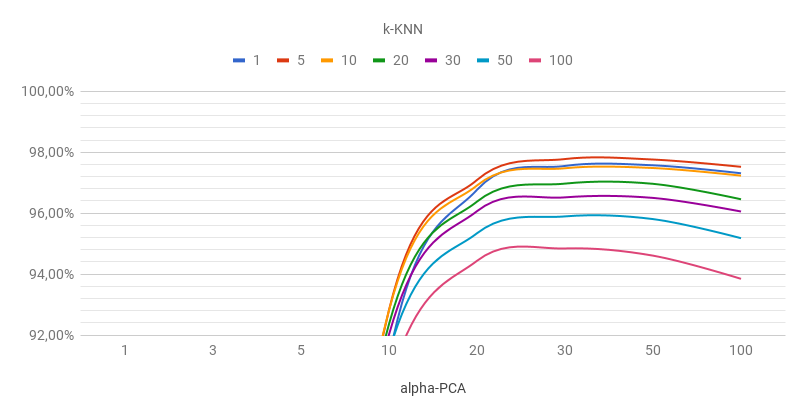
\includegraphics[width=\textwidth]{graficos/cv1_recall_zoom.png}
    \caption{Recall en función de alpha-PCA para cada k-KNN}
    \label{fig:cv1_recall_zoom}
\end{figure}

Con esta primera búsqueda se puede concluir entonces que los valores óptimos de alpha-PCA se encuentran entre 20 y 100, y los de k-KNN entre 1 y 10. Luego se realiza una segunda búsqueda más granular en estos rangos.

\subsection{Segunda búsqueda}

En esta segunda búsqueda se realizaron mediciones para alpha-PCA $20 \leq \alpha \leq 70$ y k-KNN $2 \leq \alpha \leq 8$.

\begin{figure}[h]
    \centering
    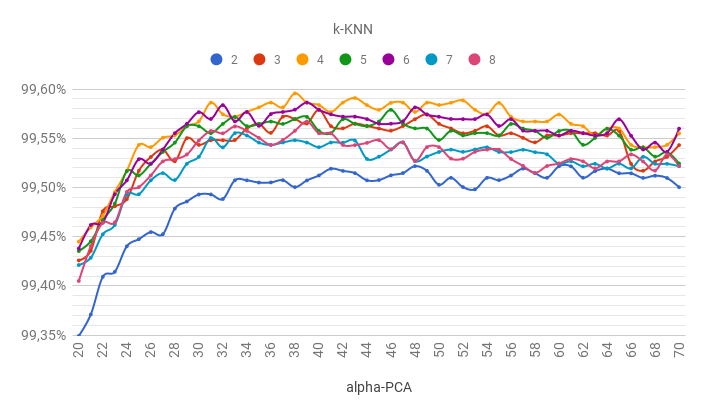
\includegraphics[width=\textwidth]{graficos/cv2_accuracy.png}
    \caption{Accuracy en función de alpha-PCA para cada k-KNN}
    \label{fig:cv2_accuracy}
\end{figure}

\begin{figure}[h]
    \centering
    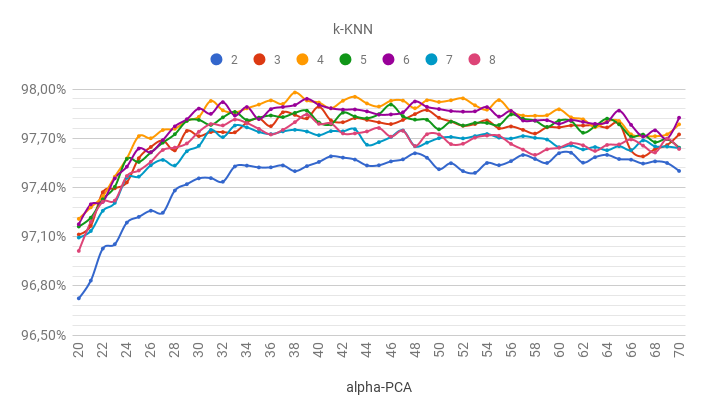
\includegraphics[width=\textwidth]{graficos/cv2_precision.png}
    \caption{Precision en función de alpha-PCA para cada k-KNN}
    \label{fig:cv2_precision}
\end{figure}

\begin{figure}[H]
    \centering
    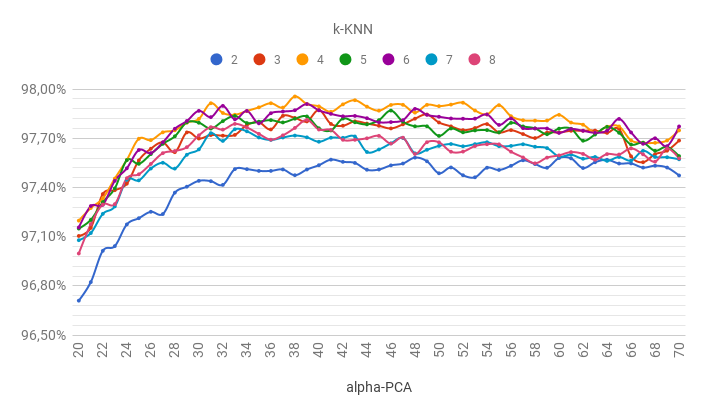
\includegraphics[width=\textwidth]{graficos/cv2_recall.png}
    \caption{Recall en función de alpha-PCA para cada k-KNN}
    \label{fig:cv2_recall}
\end{figure}

\section{Tamaño de la base de entrenamiento}

El objetivo de esta sección es analizar la relación entre el tamaño de la base de entrenamiento y el k-KNN. Para ello se realiza cross validation con 5 folds de algunos valores de k-KNN para distintas cantidades de imágenes de entrenamiento.

En este experimento se toman un total de 5000, 10000, 20000, 30000, 42000 imágenes de entrenamiento en forma aleatoria, manteniendo la misma cantidad para cada clase, y para cada una de estas cantidades se realiza cross validation con k-KNN igual a 1, 5, 10, 20, 50, 75 y 100.

El parámetro alpha se mantuvo constante al valor óptimo encontrado en la sección anterior.

\subsection{Hipótesis}

Se sabe de los experimentos anteriores que la calidad de los resultados es creciente para los primeros valores de k-KNN pero decrece a medida que siguen aumentando. Nuestra hipótesis es que se verá este comportamiento para todos los tamaños de la base de datos, pero que el decrecimiento será más pronunciado ---la pendiente tendrá una mayor magnitud--- a medida que decrece la cantidad de imágenes de entrenamiento. Esto se debe a que un valor dado de k-KNN conforma una mayor proporción en relación a la cantidad total de imágenes para tamaños pequeños que para los más grandes. Por ejemplo, un k-KNN igual a 100 constituye un $2.50\%$ de las imágenes para una base de 5000 imágenes, pero conforma sólo un $0.30\%$ de una de 42000 elementos. Esto implica que el impacto de un k-KNN malo será más grande para bases más chicas.

\subsection{Resultados}

En las figuras \ref{fig:distintos_tamanos_accuracy} y \ref{fig:distintos_tamanos_f1score} se puede ver que se cumple la hipótesis planteada ya que tanto el accuracy como el F1 score presentan un crecimiento para los valores más chicos de k-KNN pero luego decrecen, con una pendiente que crece en magnitud a medida que disminuye el tamaño de la base de entrenamiento.

\begin{figure}[h]
	\centering
	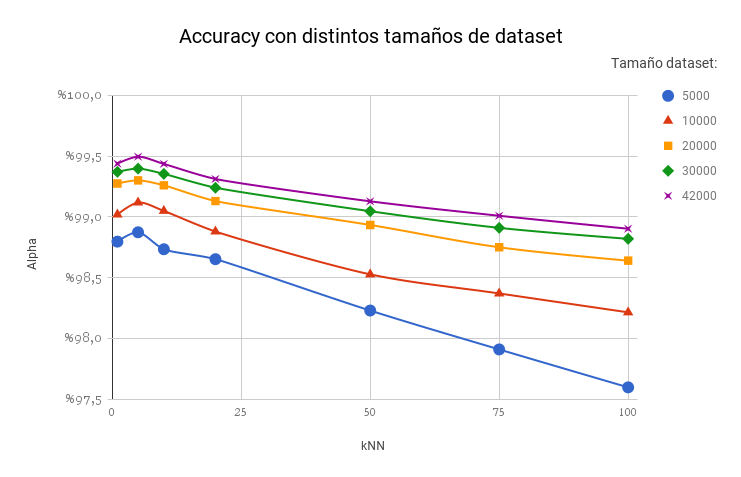
\includegraphics[width=\textwidth]{graficos/Accuracy_distintos_tamanos.png}
	\caption{Accuracy en función de k-KNN para distintos tamaños de base}
	\label{fig:distintos_tamanos_accuracy}
\end{figure}

\begin{figure}[H]
	\centering
	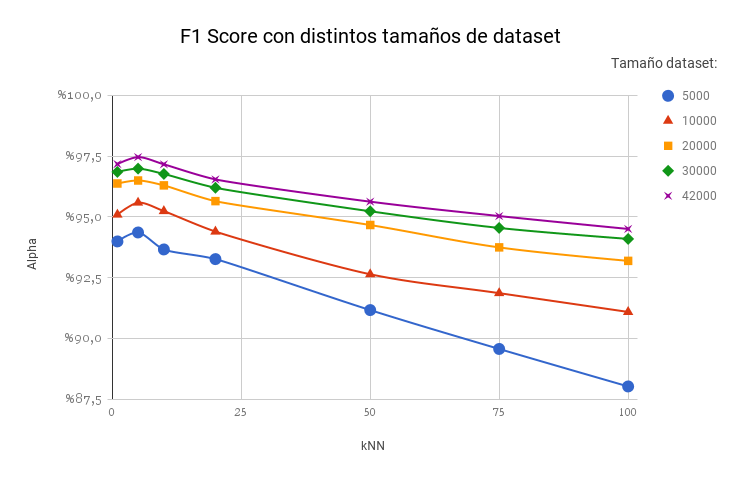
\includegraphics[width=\textwidth]{graficos/F1_score_distintos_tamanos.png}
	\caption{F1 score en función de k-KNN para distintos tamaños de base}
	\label{fig:distintos_tamanos_f1score}
\end{figure}


\section{Tiempo de ejecución}

En esta parte se hace un análisis del tiempo de ejecución del programa en función de los parámetros k-KNN y alpha-PCA.

\subsection{Hipótesis}

Con respecto a k-KNN se espera que el tiempo de ejecución tenga una relación logarítmica con respecto a su valor. Esto se debe a que en nuestra implementación los vecinos más cercanos se guardan y se actualizan en una estructura de heap, cuyo costo de inserción y borrado es logarítmico en función de la cantidad de elementos que almacena ---en este caso, a lo sumo $k$.

En cuanto a alpha-PCA la hipótesis es que afectará linealmente el tiempo de ejecución. En primer lugar, este parámetro determina la cantidad de veces que se repetirán el método de la potencia y la deflación. Por otra parte, $\alpha$ es la cantidad de filas que tendrá la matriz de cambio de base, por lo que afecta en forma lineal las operaciones de multiplicación matricial. Finalmente, a la hora de hacer KNN, $\alpha$ es la cantidad de componentes que se deberá considerar para obtener la distancia entre dos imágenes, por lo cual la complejidad de este algoritmo también es lineal en función de dicho parámetro.

\subsection{Resultados}


\section{Con PCA vs. sin PCA}

En esta sección se compara el accuracy del reconocimiento con y sin PCA para un rango de valores de k-KNN. Los valores de alpha-PCA comparados son los que se observaron como óptimos en los experimentos anteriores: 3, 4, 5 y 6.

Como se puede ver en la figura \ref{fig:cv1_sin_pca_accuracy}, el reconocimiento sin PCA presenta el mismo comportamiento con respecto a k-KNN: el accuracy crece para los valores más pequeños pero luego se mantiene en decrecimiento para valores más grandes.

Se puede observar también que los valores óptimos de k-KNN se encuentran entre 1 y 10, al igual que con el uso de PCA. Es por esta razón que la comparación entre los dos métodos se realiza para valores de k-KNN dentro de este rango.

\begin{figure}[H]
	\centering
	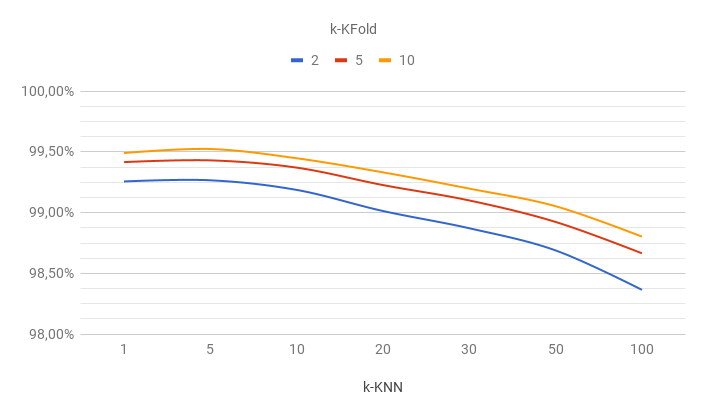
\includegraphics[width=\textwidth]{graficos/cv1_sin_pca_accuracy.png}
	\caption{Accuracy sin PCA en función de k-KNN agrupado por k-KFold}
	\label{fig:cv1_sin_pca_accuracy}
\end{figure}

\subsection{Hipótesis}

Se espera que el reconocimiento sin PCA tendrá un mejor accuracy que con el uso de PCA para cualquier $\alpha$ porque con el primer método se está utilizando toda la información disponible para determinar la cercanía de las imágenes en el algoritmo de KNN.

\subsection{Resultados}



\section{Distintos K-Fold}

En este nuevo experimento vamos a querer encontrar la relación que se encuentra entre el tamaño de $K$-fold que utilizemos y los resultados óptimos conseguidos. De esta manera usaremos nuevamente el k y el $\alpha$ que nos dio mejores resultados, pero esta vez variaremos el $K \in {2,5,8,11,15}$ de Cross validation entre los siguientes parametros . Estos fueron elegidos de esta manera ya que si utilizabamos mayores $K$ el experimento tardaria mucho mas en terminar su ejecución


\subsection{Hipótesis}

Lo que creemos que ocurrirá, a partir de los resultados obtenidos en el experimento anterior, es que con $K$ mayores el resultado se ira mejorando. La razón por la que tomamos esta hipótesis sera que a medida que sea mas grande el $K$, el set de entrenamiento será mayor. Por esto mismo se tendra mas información al decidir a que clase pertenece cada imágen.

\subsection{Resultados}

\begin{figure}
	\centering
	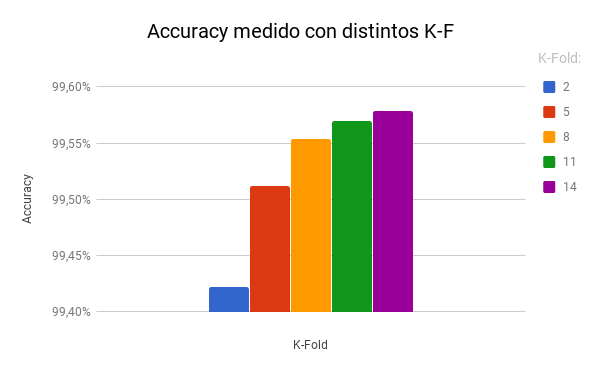
\includegraphics[width=\textwidth]{graficos/Distintos_kfold.png}
	\caption{Accuracy en función de distintos K-Fold}
	\label{fig:distintos_kfold}
\end{figure}

Finalmente se logro el resultado esperado. Como se ve en los gráficos, los resultados son mejores a partir de tener $K$ mayores, y esto se debe a que a medida que el $K$ se agranda, también se agranda la cantidad de datos de entrenamiento que se toman.

Por lo tanto de aquí podemos decir que con estos valores y utilizando toda la base de entrenamiento como tal, podemos obtener el mejor resultado, este sera el que utilizaremos en el torneo del sitio web kaggle.
